\chapter{Results}\label{Results}

\section{Model Performances}

The performance of the different random forest models IS evaluated on
the cross-validated training data with the predictions made on
telescope level.
Besides some basic performance measures, the most important features
according to the sklearn implementation are given.

\subsection{Background Separation}
\label{Gamma-/Hadron-Separation}

% The distribution of the prediction score is illustrated in figure \ref{fig:gh_sep}
% with true protons being marked in blue and true gammas in orange.

% \begin{figure}
%     \centering
%     \captionsetup{width=0.6\textwidth}
%     \includegraphics[page=2, width=.8\textwidth]{../analysis/plots/cross_val_sep_perf_plot.pdf}
%     \caption{Distribution of the predicted gammaness on the cross-validated training sets.
%         The x-axis marks the score assigned by the model.}
%     \label{fig:gh_sep}
% \end{figure}

To evaluate the resulting performance of the model, the area under the ROC-curve, precision, recall and
$F_{\num{0.1}}$-score get calculated.
The AUC is displayed in figure \ref{fig:gh_roc}.
It is almost identical for all cross-validation steps with
a mean AUC of \num{0.89}. The variations being this small is connected to the
big number of training events.

\begin{figure}
    \centering
    \captionsetup{width=0.9\linewidth}
    \hspace*{0.1\textwidth}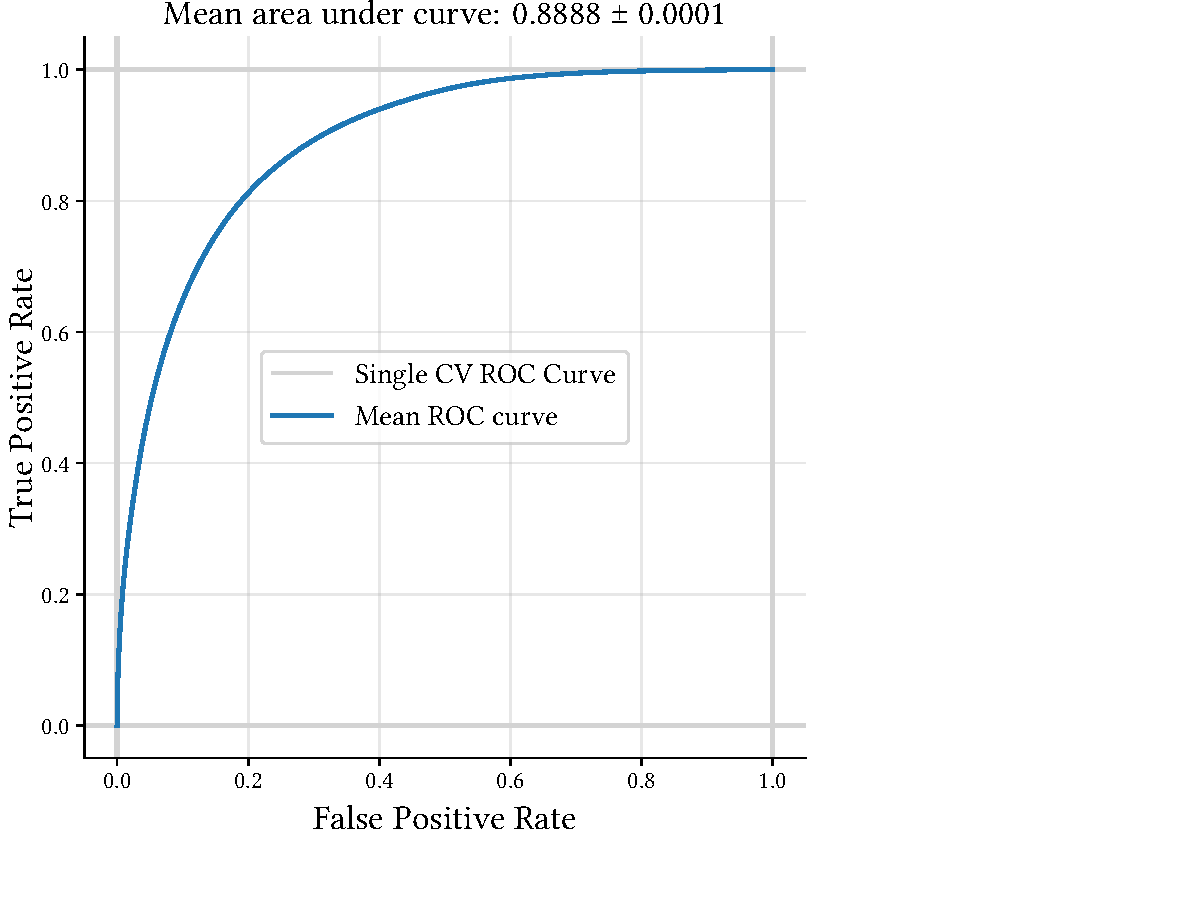
\includegraphics[page=1, width=.6\textwidth]{../analysis/plots/cross_val_sep_perf_plot.pdf}
    \caption{ROC-curve for the gamma/hadron separation on the cross-validated training sets.
    A mean AUC of \num{0.8888 \pm 0.0001} is obtained with the trained model.
    The five ROC-curves from the individual cross validation steps show almost no deviation.}
    \label{fig:gh_roc}
\end{figure}

% Figure \ref{fig:gh_fscore} shows the precision, recall and $F_{\num{0.10}}$-score over
% the prediction threshold.
% The curves for precision and recall intersect at $\approx 0.5$, visually matching the 
% results from figure \ref{fig:gh_sep}.
The other metrics can be seen in figure \ref{fig:gh_scores}.
Looking at the precision and recall, it can be noted, that no scores above 0.97 are assigned
for any sample and very few gamma events achieve scores below \num{0.1}.
The maximum of the $F_{\num{0.10}}$-score is achieved at a prediction
threshold of $\approx \num{0.8}$.

\begin{figure}
    \centering
    \captionsetup{width=0.9\textwidth}
    \includegraphics[page=3, width=.6\textwidth]{../analysis/plots/cross_val_sep_perf_plot.pdf}
    \caption{Precision, recall and $F_{\num{0.10}}$-score for the gamma/hadron separation model on the 
    cross-validated training sets.
    The precision improves up
    to $\approx \num{0.97}$ and falls to 0 above that threshold.
    This marks the highest predictions for gamma events.
    The recall on the other hand gets worse with higher threshold as legitimate gamma events,
    that achieved a low prediction, are removed and the amount of selected signal events decreases.
    The maximum $F_{\num{0.10}}$-score is achieved at a prediction threshold
    of $\approx \num{0.8}$.}
    \label{fig:gh_scores}
\end{figure}


% \begin{figure}
% 	\centering
% 	\captionsetup{width=0.6\textwidth}
% 	\begin{subfigure}{.45\textwidth}
%   		\centering
%         \hspace*{0.05\textwidth}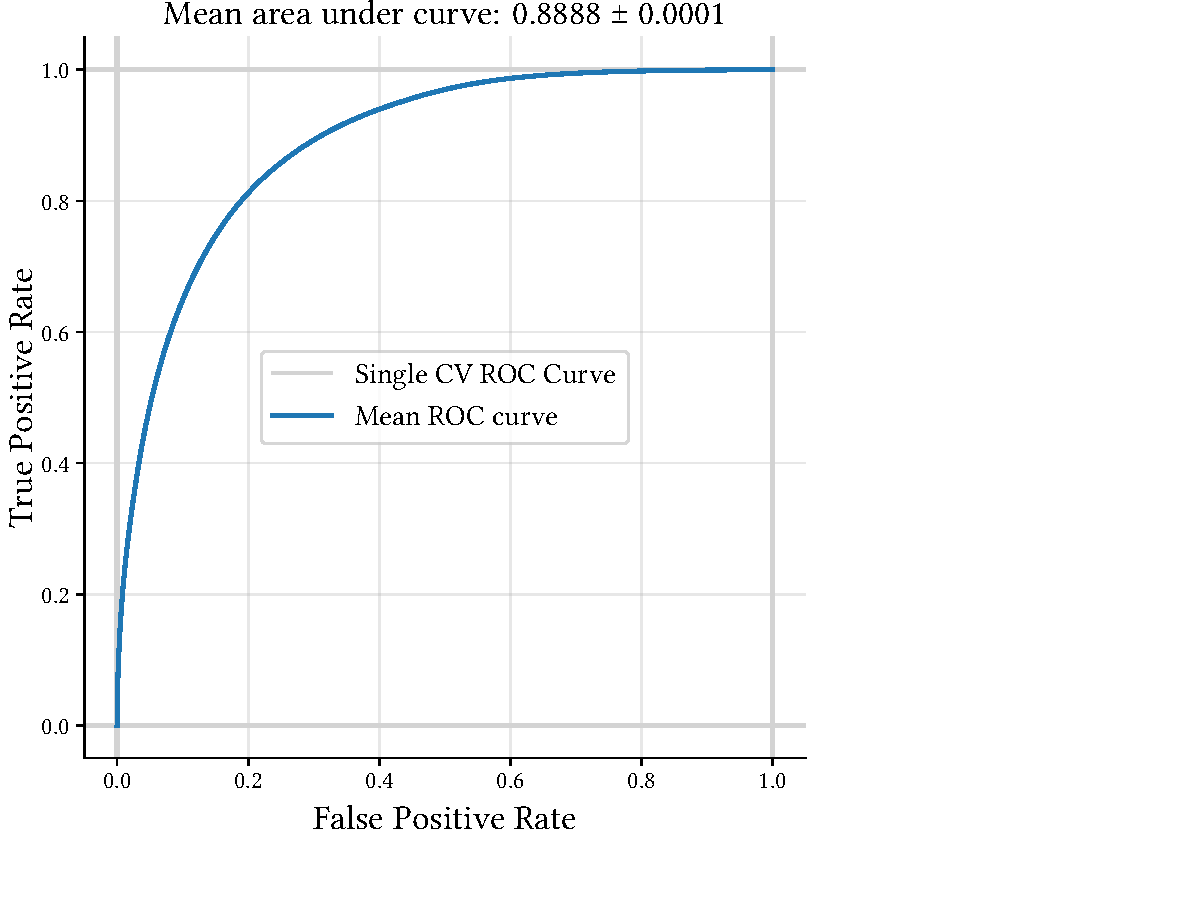
\includegraphics[page=1, width=\textwidth]{../analysis/plots/cross_val_sep_perf_plot.pdf}
% 	\end{subfigure}%
% 	\begin{subfigure}{.45\textwidth}
%  		\centering
%         \includegraphics[page=3, width=\textwidth]{../analysis/plots/cross_val_sep_perf_plot.pdf}
% 	\end{subfigure}
% 	\caption{
% 		Left: The ROC-curves for each cross validation step and the mean curve.
%         All curves are almost identical, the mean AUC achieved is \num{0.89}. \\
% 		Right: Precision, Recall and $F_{0.10}$-score. The maximum $F_{0.10}$-score
%         is achieved at a classifier threshold of $\approx 0.8$.}
% 	\label{fig:gh_eval}
% \end{figure}



The 20 most important features are listed in figure \ref{fig:gh_features}.
The individual points represent the feature importance of a single tree in one
cross-validation step, the blue line marks the median value and the box plots
contain the two inner quartiles with the whisker extending \num{1.5} times the
interquartile range.
Variation in the height of the points is added for illustration purposes and does not
contain any information.

The illustration suggests, that the separation is based mostly on the ellipsicity
and intensity concentration of the image. Additional information is gained
with the stereoscopically reconstructed features.
Timing parameters do not offer much and a distinction in different telescope types
only seems to happen to a small degree.
The $num\_islands$ feature sometimes helps with the separation.
Its distribution of feature importances shows two separated
clusters, which goes well with the discrete nature of the feature.

% Of high influence are the parameters $width$ and $width\_length$, that describe the shape of the hillas ellipse.
% The stereoscopic features $h\_max$ and $distance\_to\_reconstructed\_source\_position$ 
% provide a lot of infomation aswell.
% Also important are the parameters, that describe the intensity distribution, especially
% $log\_size\_area$ and $concentration\_cog$ and 
% in some cases also the $num\_islands$ feature.
% Timing parameters do not provide much information and the distinction in different telescope types
% does not play a big role for this task.

\begin{figure}
    \centering
    \captionsetup{width=0.9\textwidth}
    \hspace*{-0.1\textwidth}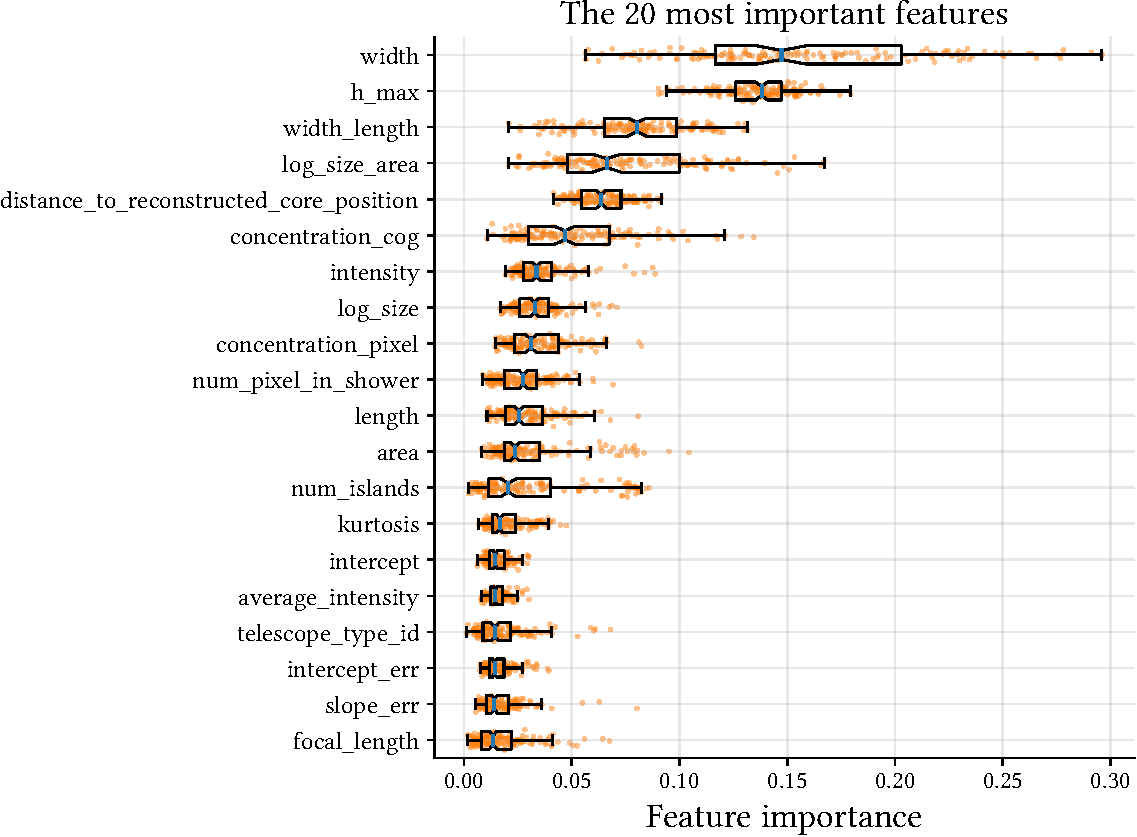
\includegraphics[page=1, width=.6\textwidth]{../analysis/plots/separation_features.pdf}
    \caption{Feature importance for the background separation model evaluated on the cross-validated dataset.
    Shown are the indvidual tree scores aswell as boxplots describing the distributions.
    The separation is based mostly on the shape of the ellipse, concentration and
    the stereoscopic features and not on timing parameters or identifying the telescope.}
    \label{fig:gh_features}
\end{figure}
